\section{Resultados}

En esta sección se muestran los tres conjuntos de resultados: el perfilado de la aplicación, el desempeño de OpenMP frente a las demás estrategias y la comparación entre las dos máquinas. Todos los tiempos están en segundos y, cuando corresponde, se reporta la \textbf{mediana} de las 10 corridas.

\subsection{Perfilado de CPU: dónde se va el tiempo}

El reporte de GProf para el kernel secuencial es concluyente:

\begin{center}
\begin{tabular}{|l|r|r|r|}
\hline
\textbf{Función} & \textbf{\% tiempo propio} & \textbf{llamadas} & \textbf{ms/llamada} \\
\hline
\texttt{multiplicar\_y\_medir} & 100.13 & 1 & 140.19 \\
\texttt{llenar\_matrices\_con\_semilla} & 0.00 & 1 & 0.00 \\
\texttt{reservar\_matrices} & 0.00 & 1 & 0.00 \\
\hline
\end{tabular}
\end{center}

El 100\% del tiempo propio de la aplicación está en la función del kernel de multiplicación, y el relleno de las matrices y la reserva de memoria son marginales. Esto confirma la decisión metodológica de cronometrar solo el kernel: es la única parte que importa.

\begin{quote}
\textbf{Advertencia sobre GProf con OpenMP.} GProf solo instrumenta el hilo principal. En la variante con OpenMP el tiempo de la región paralela se contabiliza de forma engañosa (aparece atribuido a la función que crea el equipo de hilos, no a la de trabajo real). Por eso el reporte de la variante paralela no se usa para extraer conclusiones sobre el reparto de trabajo entre hilos; para eso están los datos de Cachegrind.
\end{quote}

\subsection{Perfilado de memoria: el comportamiento de la caché}

Esta es la medición más relevante del trabajo, porque cuantifica la hipótesis que el caso de estudio 1 dejó solo como intuición. La tabla~\ref{tab:cachegrind} muestra los contadores de Cachegrind para las tres variantes del kernel, con $N=500$, medidos en la \textbf{máquina A} (Intel Core i5-12450HX, L1d de 40\,KiB por núcleo con 8 vías, L3 compartido de 12\,MiB).

\begin{table}[ht]
\centering
\scriptsize
\begin{tabular}{|l|c|r|r|r|r|r|}
\hline
\textbf{Variante} & \textbf{T} & \textbf{I refs} & \textbf{D refs} & \textbf{D1 misses} & \textbf{D1 miss rate (lect.)} & \textbf{LLd misses} \\
\hline
Secuencial (naive)  & 1  & 1\,031\,897\,709 & 389\,051\,874 & 58\,050\,493 & \textbf{22.4\%} & 48\,336 \\
Transpuesto          & 1  &   907\,904\,738 & 389\,301\,885 &  7\,893\,064 & \textbf{3.0\%}  & 48\,336 \\
OpenMP               & 1  & 1\,034\,704\,330 & 389\,325\,981 & 59\,227\,926 & 22.8\% & 48\,772 \\
OpenMP               & 8  & 1\,062\,467\,457 & 393\,297\,061 & 59\,226\,557 & 22.5\% & 49\,073 \\
OpenMP               & 16 & 1\,034\,768\,697 & 389\,344\,956 & 59\,231\,589 & 22.8\% & 49\,382 \\
\hline
\end{tabular}
\caption{Métricas de caché medidas con Cachegrind ($N=500$) en la máquina A. D1 miss rate corresponde a las lecturas de datos.}
\label{tab:cachegrind}
\end{table}

Tres observaciones se desprenden directamente de la tabla:

\begin{enumerate}
    \item \textbf{La transposición de $B$ reduce los fallos de caché L1 en un factor 7.4}: de 58.05 millones a 7.89 millones de fallos, y la tasa de fallo de lectura baja de 22.4\% a 3.0\%. Es la medición experimental de la causa del buen rendimiento del kernel transpuesto.
    \item \textbf{El número de hilos no cambia la tasa de fallo}: OpenMP con $T=1$, $T=8$ y $T=16$ dan 22.8\%, 22.5\% y 22.8\%. La tasa de fallo es una propiedad del \emph{patrón de acceso}, no del paralelismo. Esto es exactamente lo que se esperaba: el kernel con OpenMP es el mismo kernel naive, con el mismo acceso a $B$ por columna.
    \item \textbf{La transposición además reduce el número de instrucciones ejecutadas} en un 12\% (de 1\,032 millones a 908 millones), porque el acceso contiguo a $B$ es más amigable con el planificador del compilador.
\end{enumerate}

La figura~\ref{fig:cache-miss} muestra el contraste de forma visual.

\begin{figure}[ht]
\centering
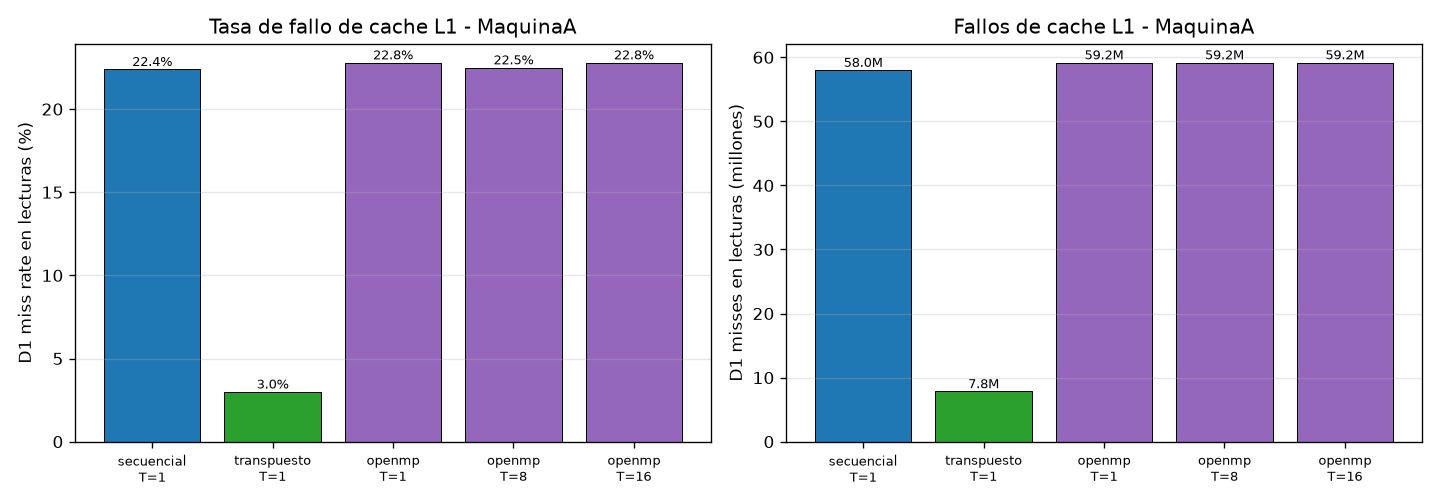
\includegraphics[width=0.95\textwidth]{figuras/cache_miss_rate.png}
\caption{Tasa de fallo de caché L1 en lecturas (izquierda) y cantidad absoluta de fallos (derecha) por variante del kernel. El kernel transpuesto (verde) reduce la tasa de fallo de 22.4\% a 3.0\%.}
\label{fig:cache-miss}
\end{figure}

\subsection{Footprint de memoria}

La memoria máxima residente (max RSS) es prácticamente idéntica en todas las variantes, como era de esperar: las tres reservan las mismas tres matrices de $N \times N$ enteros.

\begin{center}
\begin{tabular}{|l|c|r|}
\hline
\textbf{Variante} & \textbf{T} & \textbf{max RSS} \\
\hline
Secuencial (naive) & 1  & 4.4 MB \\
Transpuesto         & 1  & 4.3 MB \\
OpenMP              & 1  & 4.4 MB \\
OpenMP              & 8  & 4.5 MB \\
OpenMP              & 16 & 4.7 MB \\
\hline
\end{tabular}
\end{center}

El crecimiento con el número de hilos (de 4.4 a 4.7 MB) corresponde al \emph{overhead} de las pilas de hilo y de las estructuras de control del \textit{runtime} de OpenMP, que es de apenas unos cientos de kilobytes. La figura~\ref{fig:rss} lo muestra.

\begin{figure}[ht]
\centering
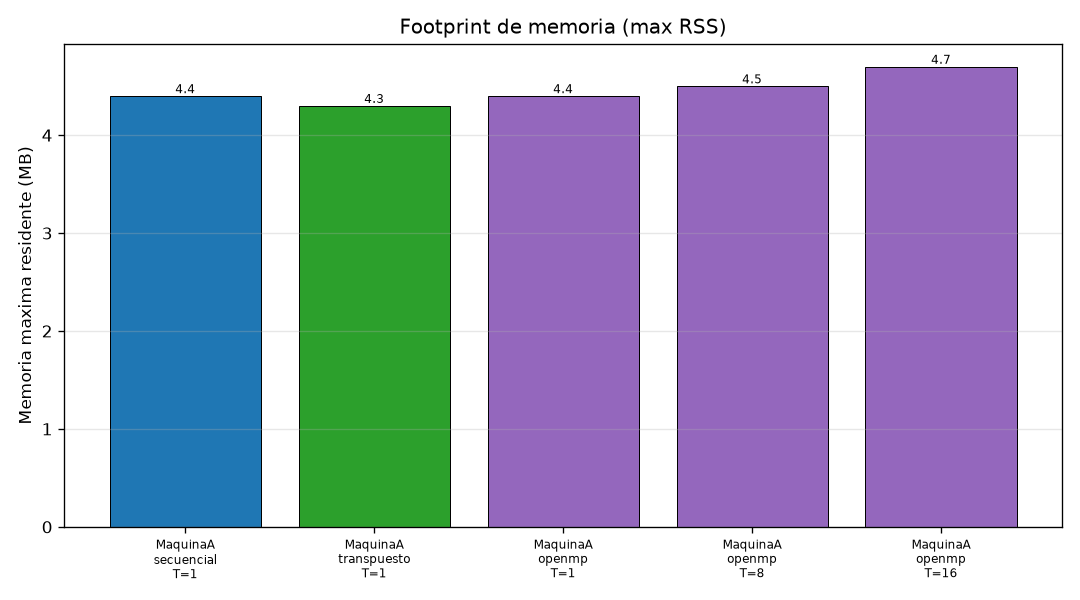
\includegraphics[width=0.7\textwidth]{figuras/footprint_memoria.png}
\caption{Footprint de memoria (max RSS) por variante del kernel.}
\label{fig:rss}
\end{figure}

\subsection{Desempeño: las cinco estrategias comparadas}

La tabla~\ref{tab:cinco-estrategias} compara las cinco estrategias sobre la misma base secuencial. Para OpenMP se reporta el mejor $T$ por $N$, que es la misma metodología que se aplicó a pthreads y a fork.

\begin{table}[ht]
\centering
\small
\begin{tabular}{|c|r|r|r|r|r|r|}
\hline
\textbf{N} & \textbf{T\_seq} & \textbf{T\_pth} & \textbf{T\_fork} & \textbf{T\_full} & \textbf{T\_mem} & \textbf{T\_omp} \\
\hline
500  & 0.0440 & 0.0315 (T=16) & 0.0152 (T=8) & 0.0459 & 0.0377 & 0.0160 (T=16) \\
1000 & 0.4230 & 0.2043 (T=16) & 0.1169 (T=16) & 0.4301 & 0.3019 & 0.1179 (T=16) \\
2000 & 4.3626 & 1.6430 (T=16) & 1.9805 (T=8) & 5.8909 & 2.6586 & 1.2786 (T=16) \\
4000 & 75.6511 & 24.2927 (T=16) & 59.1421 (T=8) & 70.0332 & 21.3223 & 16.6689 (T=8) \\
\hline
\end{tabular}
\caption{Tiempos (s, mediana de 10 corridas) de las cinco estrategias. La base es el secuencial con $-O2$. Entre paréntesis se indica el mejor $T$ de cada estrategia paralela.}
\label{tab:cinco-estrategias}
\end{table}

\begin{table}[ht]
\centering
\small
\begin{tabular}{|c|r|r|r|r|r|}
\hline
\textbf{N} & \textbf{s\_pth} & \textbf{s\_fork} & \textbf{s\_full} & \textbf{s\_mem} & \textbf{s\_omp} \\
\hline
500  & 1.40 & 2.89 & 0.96 & 1.17 & \textbf{2.75} \\
1000 & 2.07 & 3.62 & 0.98 & 1.40 & \textbf{3.59} \\
2000 & 2.66 & 2.20 & 0.74 & 1.64 & \textbf{3.41} \\
4000 & 3.11 & 1.28 & 1.08 & 3.55 & \textbf{4.54} \\
\hline
\end{tabular}
\caption{Speedup de las cinco estrategias respecto al secuencial.}
\label{tab:speedups}
\end{table}

\begin{figure}[ht]
\centering
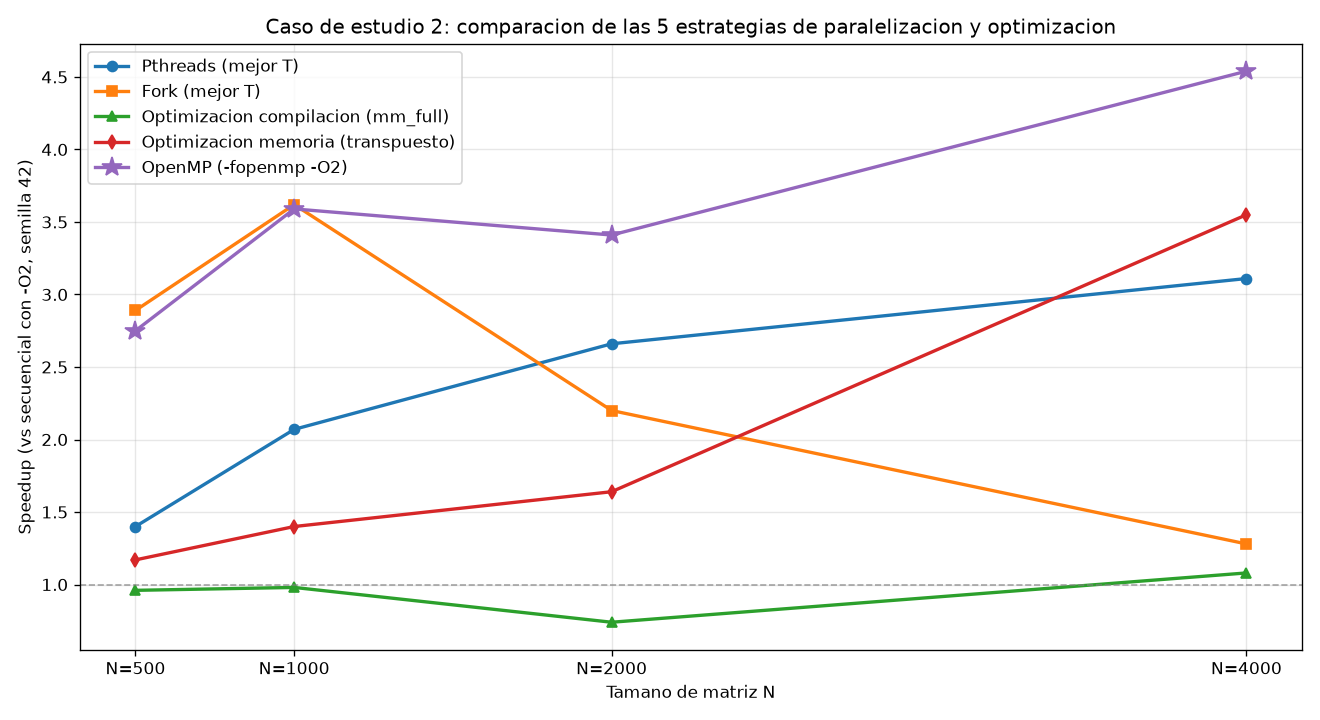
\includegraphics[width=0.95\textwidth]{figuras/comparativa_5_estrategias.png}
\caption{Speedup de las cinco estrategias frente al secuencial. OpenMP (estrella morada) es la estrategia más rápida en tres de los cuatro tamaños.}
\label{fig:5-est}
\end{figure}

\subsection{Escalamiento de OpenMP}

El detalle por cantidad de hilos muestra el comportamiento interno del paralelismo:

\begin{table}[ht]
\centering
\begin{tabular}{|c|r|r|r|r|r|c|}
\hline
\textbf{N} & \textbf{T=1} & \textbf{T=2} & \textbf{T=4} & \textbf{T=8} & \textbf{T=16} & \textbf{Speedup} \\
\hline
500  & 0.0450 & 0.0276 & 0.0239 & 0.0180 & \textbf{0.0160} & 2.81$\times$ \\
1000 & 0.4257 & 0.2385 & 0.1652 & 0.1473 & \textbf{0.1179} & 3.61$\times$ \\
2000 & 4.3026 & 2.7034 & 1.5880 & 1.4391 & \textbf{1.2786} & 3.36$\times$ \\
4000 & 76.0226 & 34.3422 & 18.0106 & \textbf{16.6689} & 18.0214 & 4.56$\times$ \\
\hline
\end{tabular}
\caption{Tiempos (s) de OpenMP por cantidad de hilos y speedup resultante respecto al $T=1$ de la misma máquina.}
\label{tab:escalamiento}
\end{table}

Dos detalles merecen atención. Primero, el $T=16$ \emph{empeora} frente al $T=8$ para $N=4000$ (18.02\,s contra 16.67\,s): la máquina tiene 12 núcleos lógicos, de modo que 16 hilos obligan al sistema a planificar más trabajo del que puede ejecutar en paralelo, y el \emph{overhead} de esa planificación se come la ganancia. Segundo, el $T=1$ de OpenMP (76.02\,s) es prácticamente igual al secuencial de referencia (75.65\,s): con un solo hilo, OpenMP no aporta nada pero tampoco cuesta nada, lo que confirma que el speedup de 4.56$\times$ se debe \emph{exclusivamente} al paralelismo y no a diferencias de compilación.

\subsection{Comparación entre las dos máquinas}

\textit{[Pendiente de completar con la segunda máquina. Se deja la tabla y las gráficas listas para ser rellenadas con los resultados del segundo equipo.]}

La máquina A, sobre la que se corrieron las mediciones de la tabla~\ref{tab:cinco-estrategias}, es:

\begin{center}
\begin{tabular}{|l|l|}
\hline
\textbf{Característica} & \textbf{Valor} \\
\hline
CPU & Intel Core i5-12450HX (12\textsuperscript{a} generación, Alder Lake) \\
Núcleos físicos / lógicos & 8 / 12 (hyperthreading) \\
Caché L1d / L2 / L3 & 320 KiB / 7 MiB / 12 MiB \\
Memoria RAM & 15 GiB \\
Sistema operativo & Debian GNU/Linux 13 (trixie), kernel 6.12.74 \\
Compilador & gcc 14.2.0 \\
Flags & \texttt{-Wall -O2 -fopenmp} \\
\hline
\end{tabular}
\end{center}

\begin{table}[ht]
\centering
\begin{tabular}{|c|c|r|c|r|c|r|}
\hline
\textbf{N} & \textbf{Máquina} & \textbf{T\_opt} & \textbf{T\_opt (s)} & \textbf{T=1 (s)} & \textbf{Speedup interno} & \textbf{\%$\Delta$ vs A} \\
\hline
500  & A & 16 & 0.0160 & 0.0450 & 2.81$\times$ & --- \\
500  & B & \textit{(completar)} & & & & \\
1000 & A & 16 & 0.1179 & 0.4257 & 3.61$\times$ & --- \\
1000 & B & \textit{(completar)} & & & & \\
2000 & A & 16 & 1.2786 & 4.3026 & 3.36$\times$ & --- \\
2000 & B & \textit{(completar)} & & & & \\
4000 & A & 8  & 16.6689 & 76.0226 & 4.56$\times$ & --- \\
4000 & B & \textit{(completar)} & & & & \\
\hline
\end{tabular}
\caption{Comparación entre máquinas. La columna $\%\Delta$ indica cuánto mayor (o menor) es el rendimiento de la máquina A respecto de la B, según $R=1/T$.}
\label{tab:benchmark-maquinas}
\end{table}

\begin{figure}[ht]
\centering
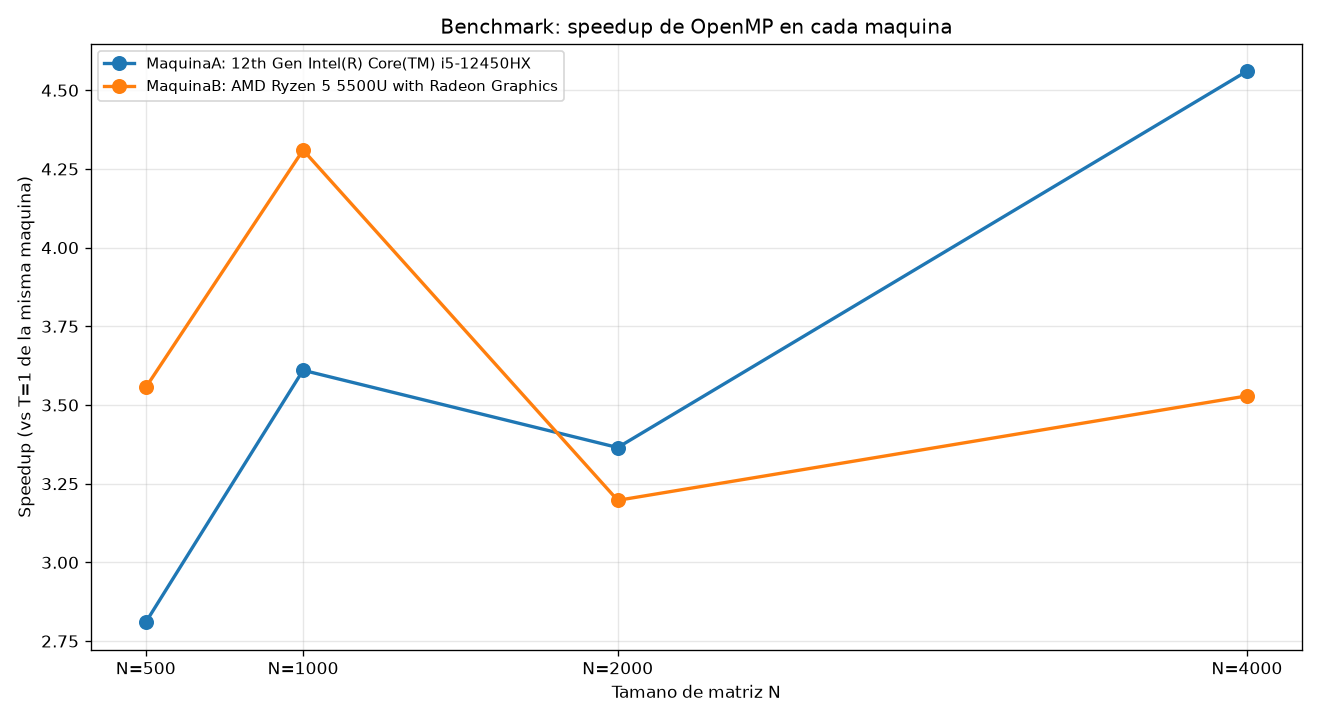
\includegraphics[width=0.9\textwidth]{figuras/benchmark_maquinas.png}
\caption{Speedup interno de OpenMP en cada máquina.}
\label{fig:benchmark-maquinas}
\end{figure}

\begin{figure}[ht]
\centering
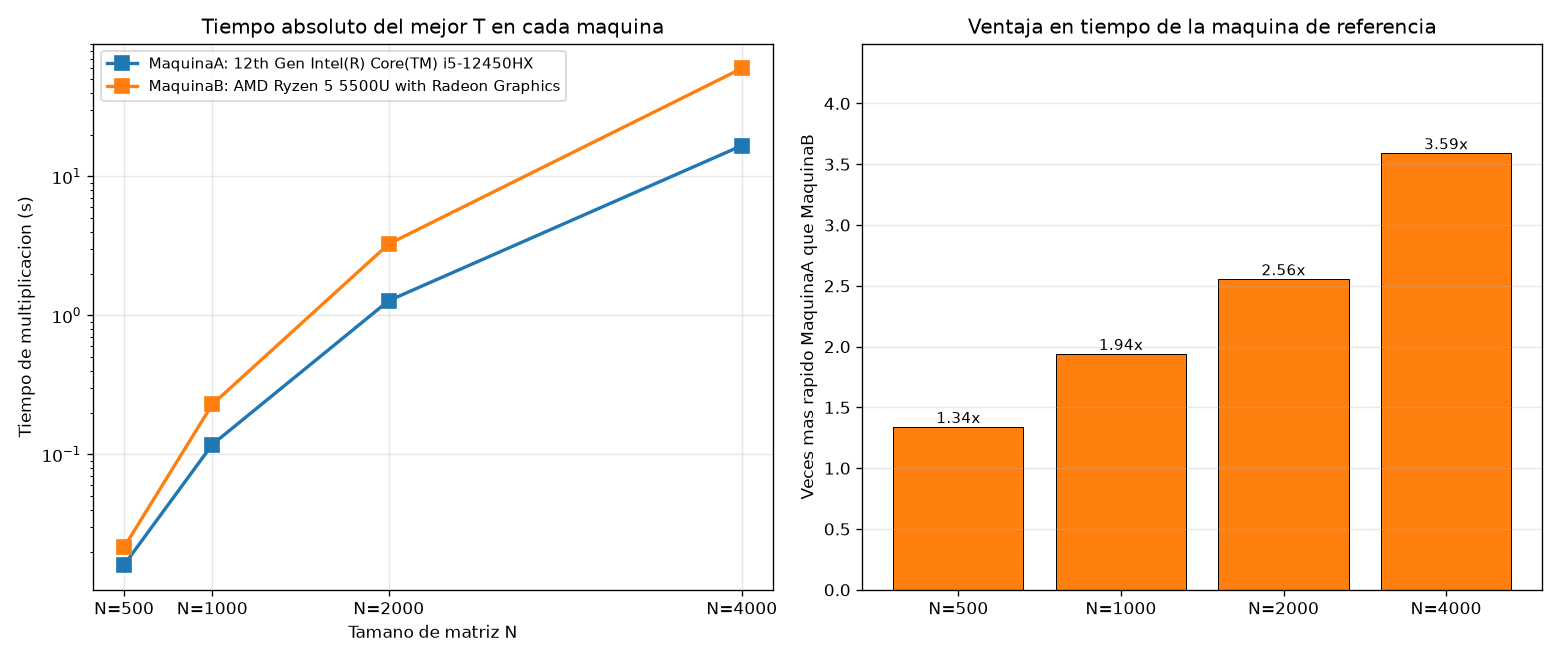
\includegraphics[width=0.9\textwidth]{figuras/benchmark_tiempos.png}
\caption{Tiempo absoluto del mejor $T$ en cada máquina (escala logarítmica).}
\label{fig:benchmark-tiempos}
\end{figure}

\begin{figure}[ht]
\centering
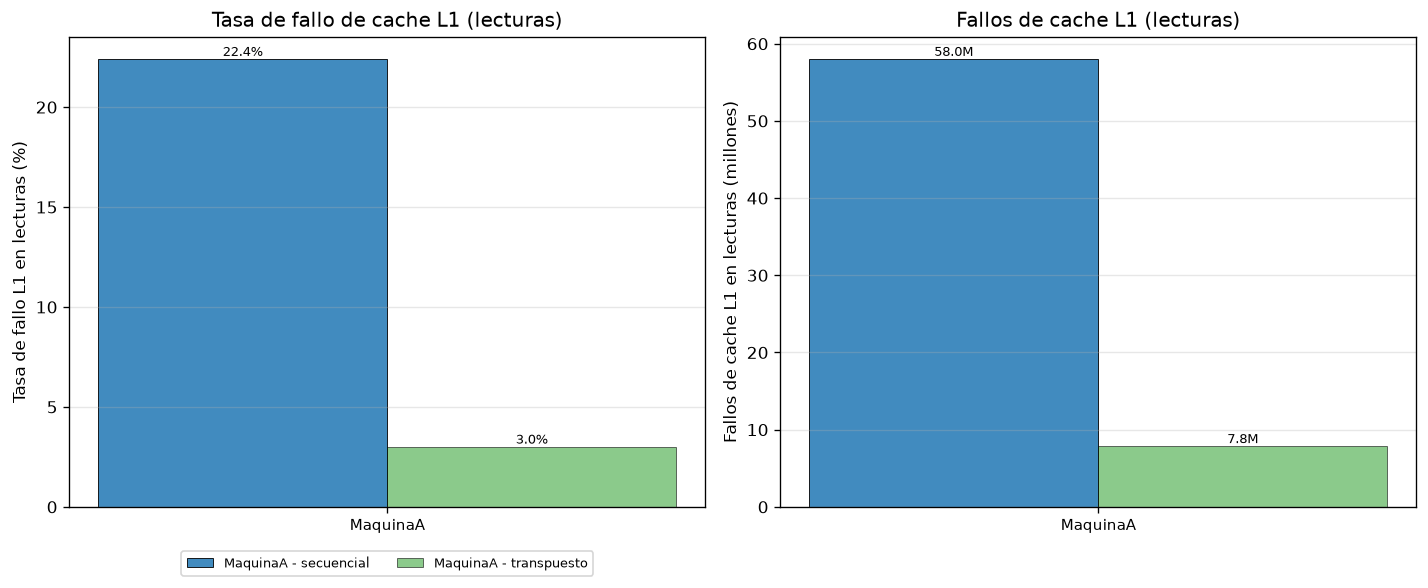
\includegraphics[width=0.95\textwidth]{figuras/cache_miss_rate_maquinas.png}
\caption{Tasa de fallo de caché L1 y fallos absolutos, comparando el kernel naive con el transpuesto en cada máquina. Como Cachegrind simula la caché real del equipo, estas cifras son distintas en cada hardware.}
\label{fig:cache-maquinas}
\end{figure}
